%% vi: set tabstop=2, set textwidth=80

\documentclass[11pt]{article}

\usepackage{homework}
\usepackage{graphicx}
\usepackage{algorithm}
\usepackage{algorithmic}
\usepackage{amsmath, amsthm, amssymb}
\usepackage{subfigure}
\usepackage[english]{babel}

% The report should be a description of your work during the lab sessions,
% focussing on the mean shift tracker. You should describe what you did, what you
% noticed and what you could have done different or could have improved. As you
% implemented the tracker you noticed different behaviour if you changed parts of
% the tracker, e.g. a different colour space or the number of bins in the
% histogram. Hopefully these insights have improved your tracker. This is why it
% is essential that you test the tracker also on a video of a domain other than
% soccer (or any other sport on a green field). This other domain will show how
% your implementation depends on the soccer domain. Observe how you can improve
% your design and them describe how you implemented this change or, for lack of
% time, describe how you would change your design. 

\title{Intelligent Multimedia Systems \\ Mean Shift Tracker}

\author{F. Huizinga [0418862], B. Stoeller [0426857] \\
      \{folkerthuizinga,bramstoeller\}@gmail.com}

\date{December 27, 2009}

\begin{document}
\maketitle

\begin{abstract}
This report describes the implementation and results of a mean shift tracker
using the Epanechnikov kernel and various color space models. Furthermore we
perform some analysis on the tracker and color models with the use of two
videos within different domains.
\end{abstract}


\section{Introduction}
An object tracker consists of two major components, the \emph{Object Model} and
the \emph{Tracking Algorithm}. The object model is represented using a
histogram in some color space. The tracking algorithm is the Mean Shift
Algorithm~\cite{kernel-basedobject, real-timetracking}. This report compares
six different color spaces to represent the Object Model and their performance
is measured using two videos in different domains (sport and nature). The
report is organized as follows.  Section 2 describes the implementation of the
algorithm. The experiments and results are shown in Section 3. Section 4
presents our conclusions, and finally possible improvements are shown in
Section 5. \newpage


\section{Implementation}
For our implementation we used the Matlab programming language. We describe the
implementation of the tracking algorithm and the object model seperatly.

\subsection{Object Model}
The object model is represented as a 2D or 3D histogram on the following color
spaces: rgb, xyz, RGB, HSI and XYZ. We decided to use a fixed number of total
bins (i.e. the number of bins is not affected by the number of dimensions).
More precise, if $N$ is the total number of bins, then the number of bins $b$
for each dimension $i$ is $b_i = N^{1/d}$, where $d$ is the total number of
dimensions. 

\subsection{Tracking Algorithm}
Algorithm \ref{alg:mst} shows our toplevel implementation of the mean shift
tracking algorithm, for the complete details we refer the reader to the
enclosed (documented) sourcecode.
\begin{algorithm}
	\caption{MeanShiftTracker($V$, $n$)}
	\begin{algorithmic}[1]
	\REQUIRE The video $V$ with $n$ frames
	\STATE $f_1 \leftarrow V[1]$ \COMMENT{Set the current frame}
	\STATE $\mathbf{y_0} \leftarrow \mathcal{S}(f_1)$ \COMMENT{Select target, store location}
	\STATE $\mathbf{q} \leftarrow \mathcal{M}(f_1, \mathbf{y_0})$ \COMMENT{Create the target model}
	\FOR{$i = 1$ to $n$}
		\STATE $f_i \leftarrow V[i]$
		\STATE $\mathbf{p_0} \leftarrow \mathcal{M}(f_i, \mathbf{y_0})$
		\STATE $bc_0 \leftarrow \mathcal{B}(\mathbf{p_0}, \mathbf{q})$ \COMMENT{Compute Bhattacharyya coefficient}
		\WHILE{true}
			\STATE $\mathbf{W} \leftarrow \mathcal{W}(f_i, \mathbf{y_0}, \mathbf{q}, \mathbf{p_0})$ \COMMENT{Compute the weights matrix}
			\STATE $\mathbf{y_1} \leftarrow \mathbf{y_0} + \mathcal{L}(\mathbf{W})$ \COMMENT{Compute the mean shift}
			\STATE $\mathbf{p_1} \leftarrow \mathcal{M}(f_i, \mathbf{y_1})$
			\STATE $bc_1 \leftarrow \mathcal{B}(\mathbf{p_1}, \mathbf{q})$
			\WHILE{$bc_1 < bc_0$} 
				\STATE $\mathbf{y_1} \leftarrow \frac{1}{2} \dot (\mathbf{y_0} + \mathbf{y_1})$ \COMMENT{Interpolate $\mathbf{y_1}$ if we shifted too far}
				\STATE $\mathbf{p_1} \leftarrow \mathcal{M}(f_i, \mathbf{y_1})$
				\STATE $bc_1 \leftarrow \mathcal{B}(\mathbf{p_1}, \mathbf{q})$
			\ENDWHILE
			\STATE $\mathbf{p_0} \leftarrow \mathbf{p_1}$
			\STATE $\mathbf{y_0} \leftarrow \mathbf{y_1}$
			\STATE $bc_0 \leftarrow bc_1$
			\IF{$\| \mathbf{y_1} - \mathbf{y_0} \| < \epsilon$}
				\STATE break \COMMENT{Break if locations are nearly equal}
			\ENDIF
		\ENDWHILE
	\ENDFOR
	\medskip
	\end{algorithmic}
\label{alg:mst}
\end{algorithm}


\section{Experiments and Results}
For our experiments we applied the tracker to videos within two different
domains, nature and sports. Figure \ref{fig:videos} shows the tracker in action
on both domains. 
\begin{figure}[!ht]
\centering
\subfigure[The sports domain, a soccer match.]{
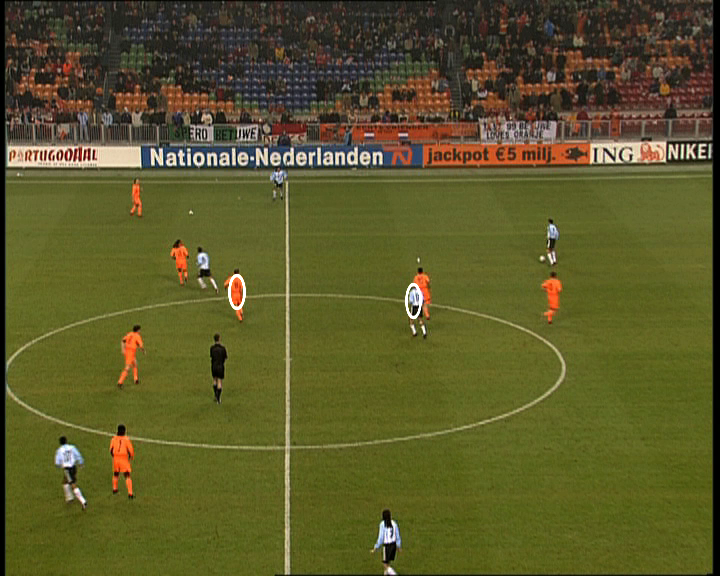
\includegraphics[height=5.0cm]{img/soccer}
\label{fig:a}
}
\subfigure[The nature domain, a hunting cheetah.]{
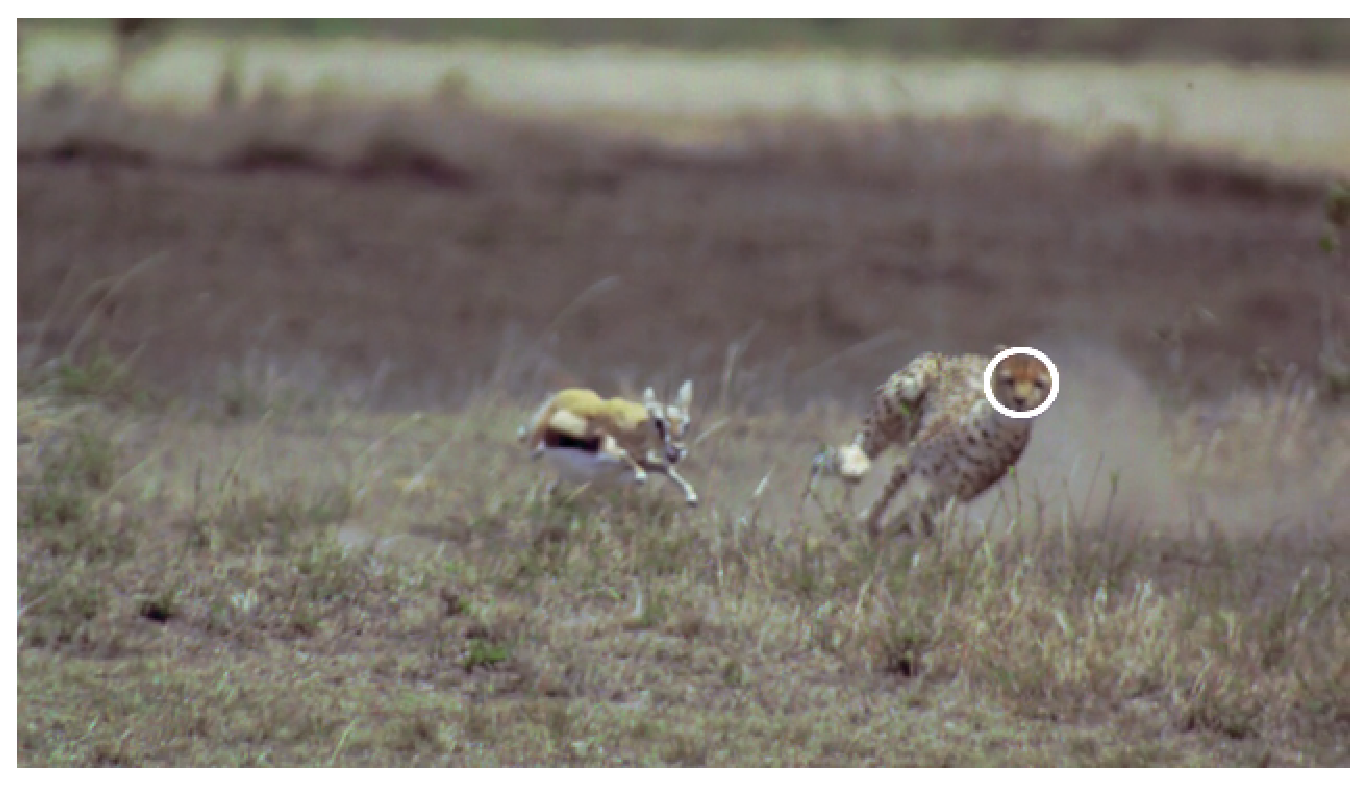
\includegraphics[height=5.0cm]{img/earth_cheetah_scene}
\label{fig:b}
}
\caption{\ref{fig:a} shows the sport domain where we track an orange soccer
player on the left. \ref{fig:b} shows a scene from the movie Earth, where we
track the head of a cheetah chasing its prey.}
\label{fig:videos}
\end{figure}
In both videos a distinctive object was tracked using the various color models
and for each color model various histogram sizes, see Table \ref{table:bins}.
\begin{table}[!ht]
\centering
\begin{tabular}{l|l|l}
$N$     & $N^{1/2}$ & $N^{1/3}$\\\hline
$64$    & $8$       & $4$\\\hline
$729$   & $27$      & $9$\\\hline
$4096$  & $64$      & $16$\\\hline
$15625$ & $125$     & $25$\\
\end{tabular}
\caption{Histogram sizes.}
\label{table:bins}
\end{table}
For an (somewhat) objective analysis of the various colormodels and various
histogram sizes, we chose to manually tag the objects within the frame
sequences of each video. Figures \ref{fig:cheetah} and \ref{fig:soccer} show
our final results for the tracking of the cheetah's head and orange soccer
player respectively.  
Both figures show four graphs with the frame number on the $x$-axis and the
euclidian distance, between the tracker's output and our labelled data, on the
$y$-axis. Each of the four graphs corresponds to a certain total number of
bins. From these results we can see that the $rgb$ model is the only model that
doesn't fail in all of the cases. This indicates that the $rgb$ colormodel is a
robust one and would indeed be our choice for object tracking.
\begin{figure}[!ht]
\centering
\subfigure[$64$ bins]{
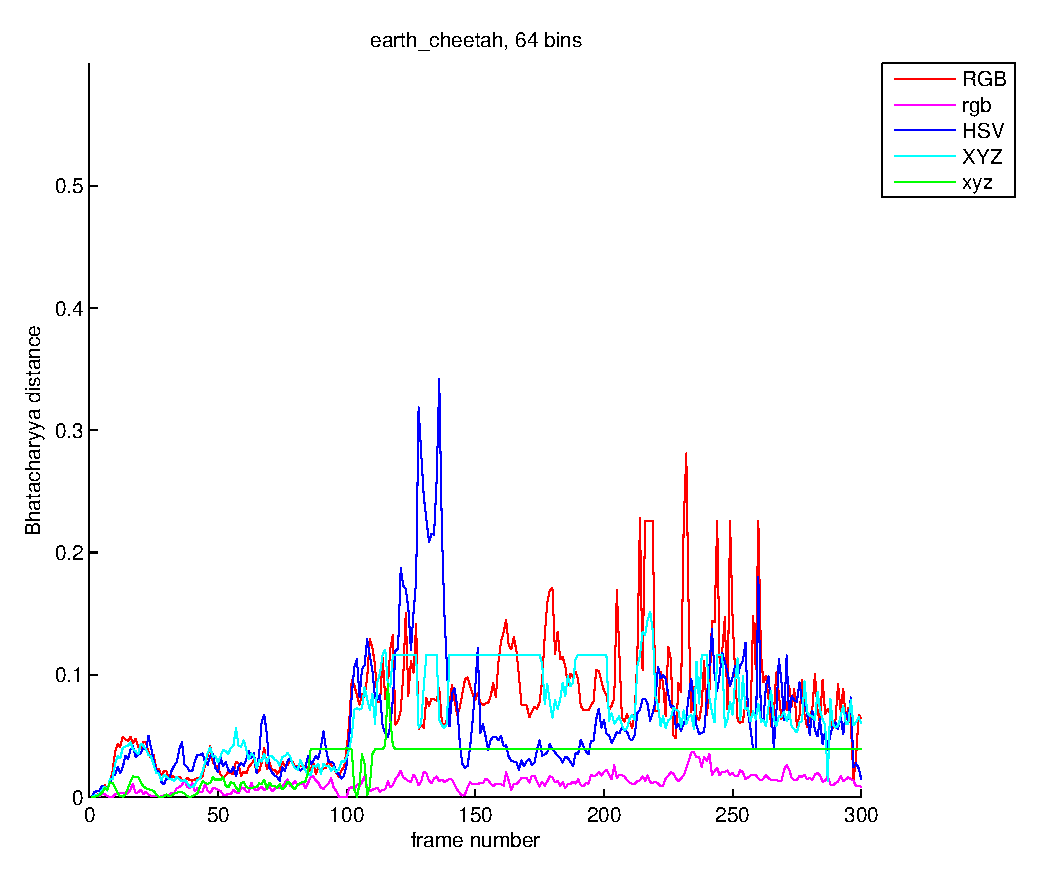
\includegraphics[height=6.0cm]{img/earth_cheetah_64}
\label{fig:a}
}
\subfigure[$729$ bins]{
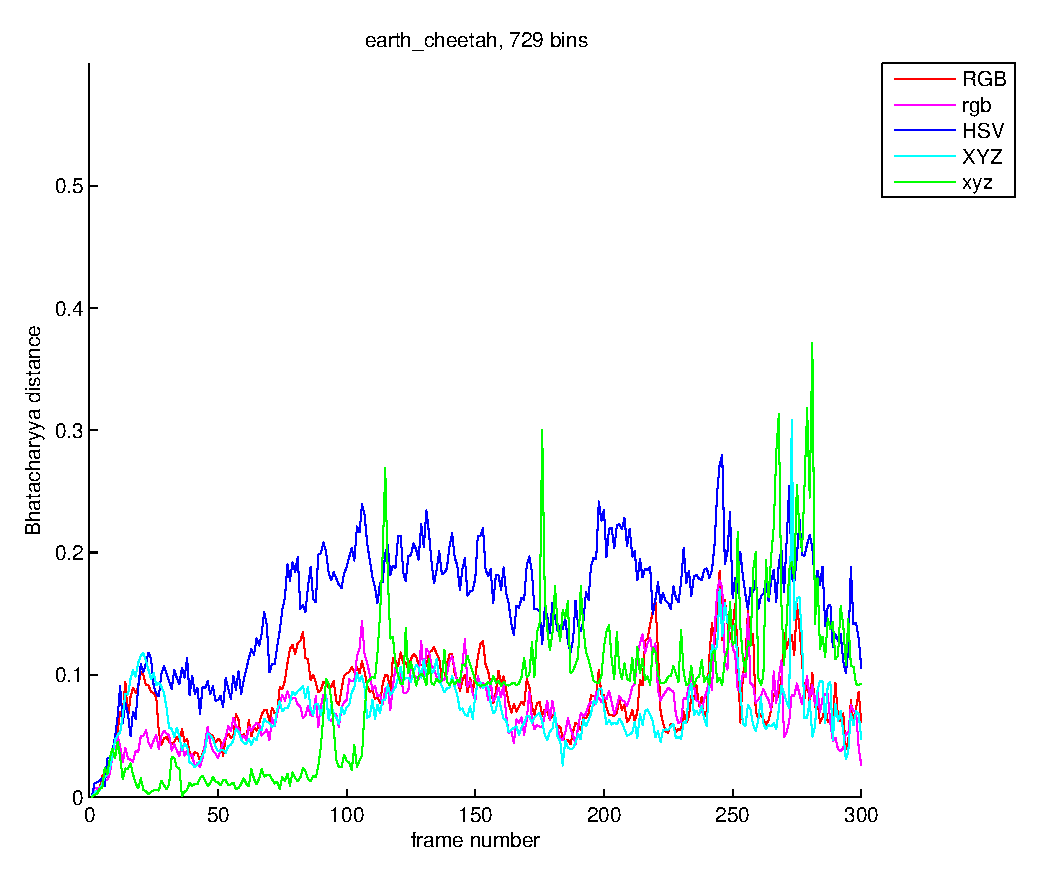
\includegraphics[height=6.0cm]{img/earth_cheetah_729}
\label{fig:b}
}
\\
\subfigure[$4096$ bins]{
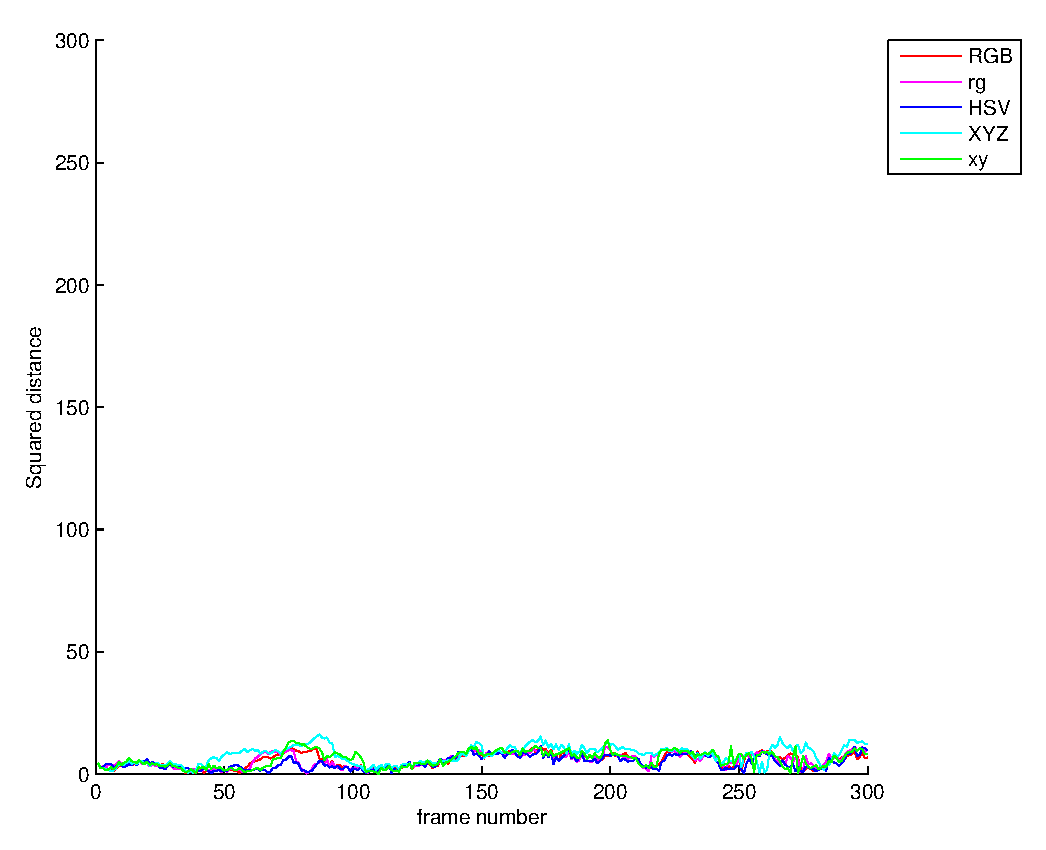
\includegraphics[height=6.0cm]{img/earth_cheetah_4096}
\label{fig:c}
}
\subfigure[$15625$ bins]{
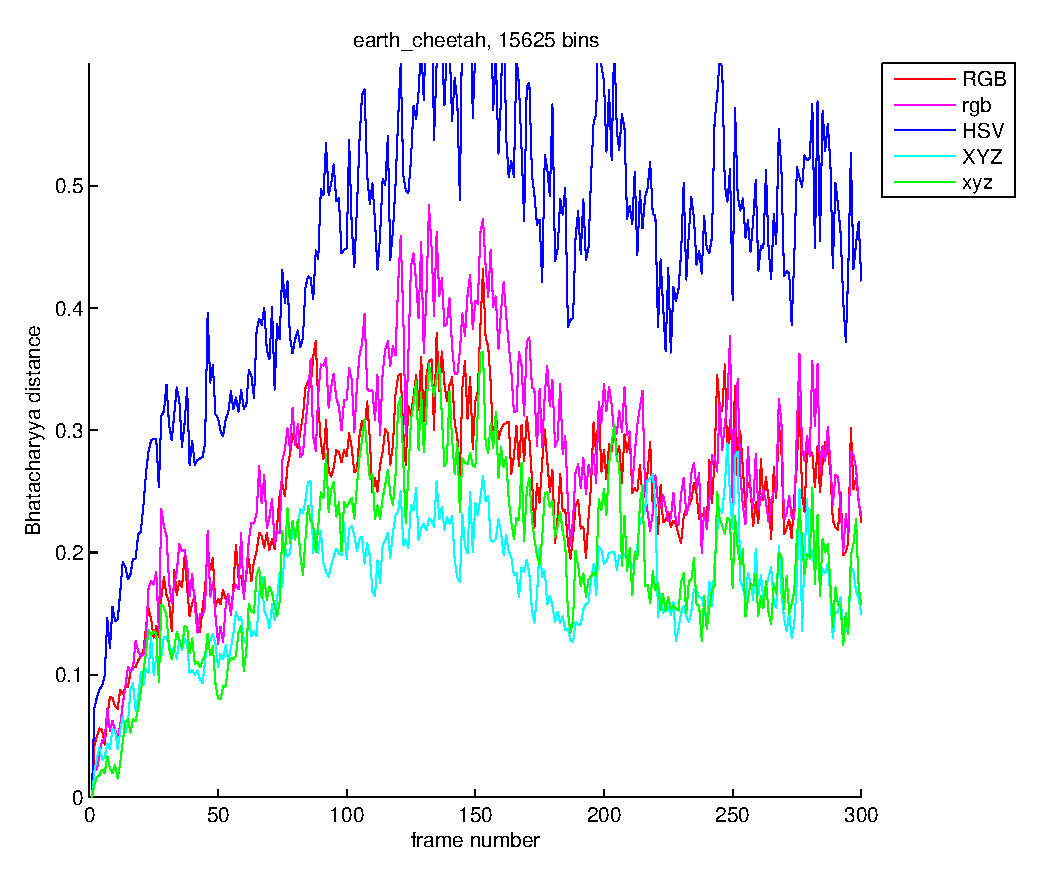
\includegraphics[height=6.0cm]{img/earth_cheetah_15625}
\label{fig:d}
}
\caption{Each graph shows the performance of the six different colormodels for
a number of bins on the cheetah movie when tracking the cheetah's head.
\ref{fig:a} shows that several colormodels have completely lost track,
indicating that $64$ is not enough. In \ref{fig:b} just the $xyz$ model failed.
Both \ref{fig:c} and \ref{fig:d} all colormodels show good performance.
Indicating that the more bins used, the better the model becomes.}
\label{fig:cheetah}
\end{figure}

\begin{figure}[!ht]
\centering
\subfigure[$64$ bins]{
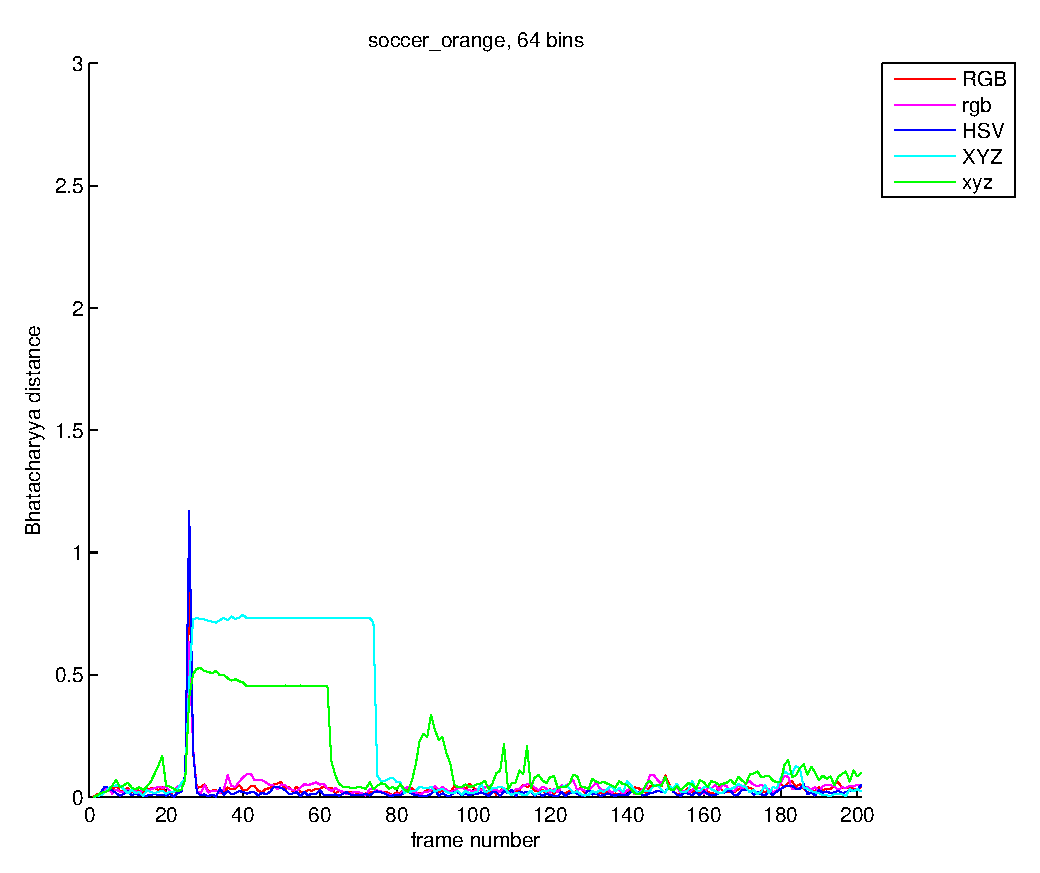
\includegraphics[height=6.0cm]{img/soccer_orange_64}
\label{fig:a}
}
\subfigure[$729$ bins]{
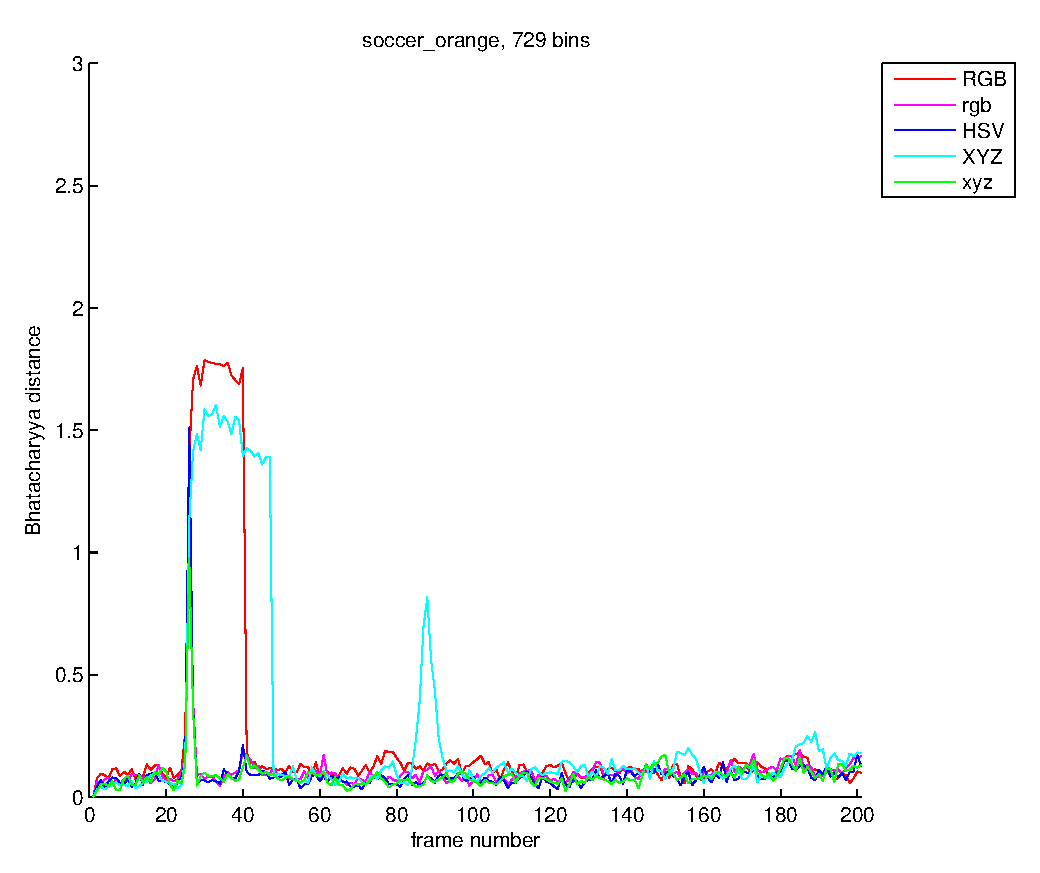
\includegraphics[height=6.0cm]{img/soccer_orange_729}
\label{fig:b}
}
\\
\subfigure[$4096$ bins]{
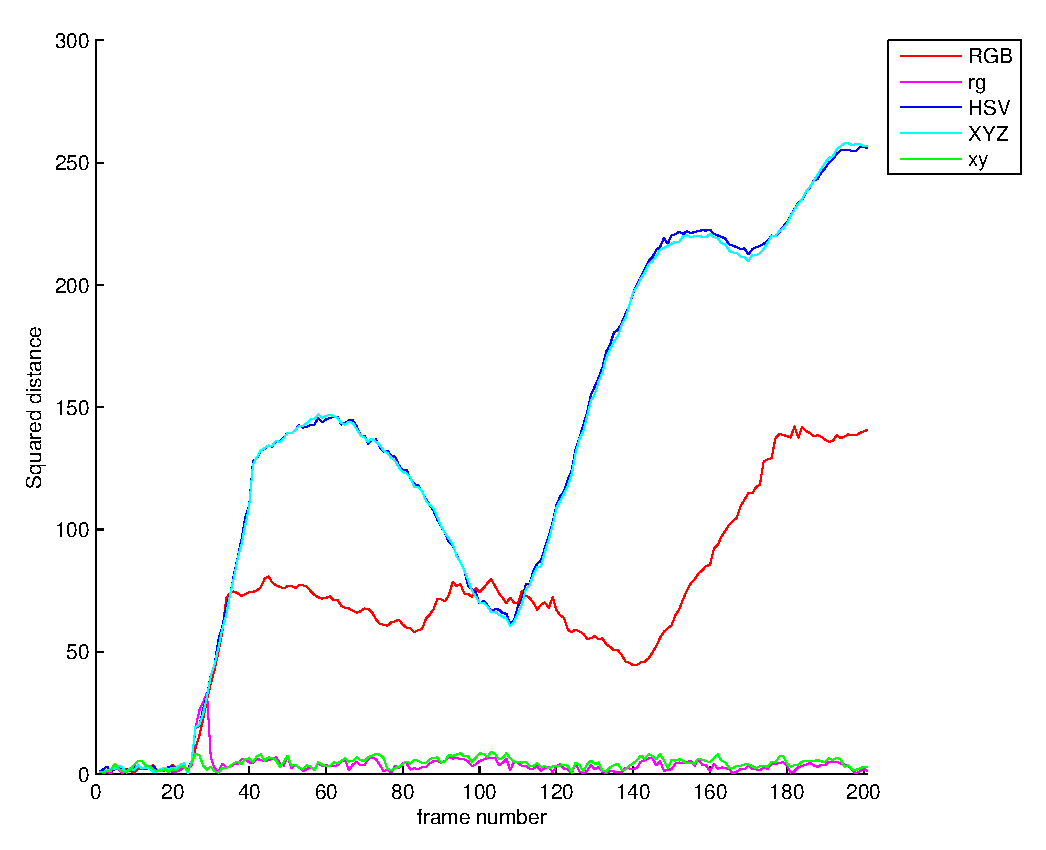
\includegraphics[height=6.0cm]{img/soccer_orange_4096}
\label{fig:c}
}
\subfigure[$15625$ bins]{
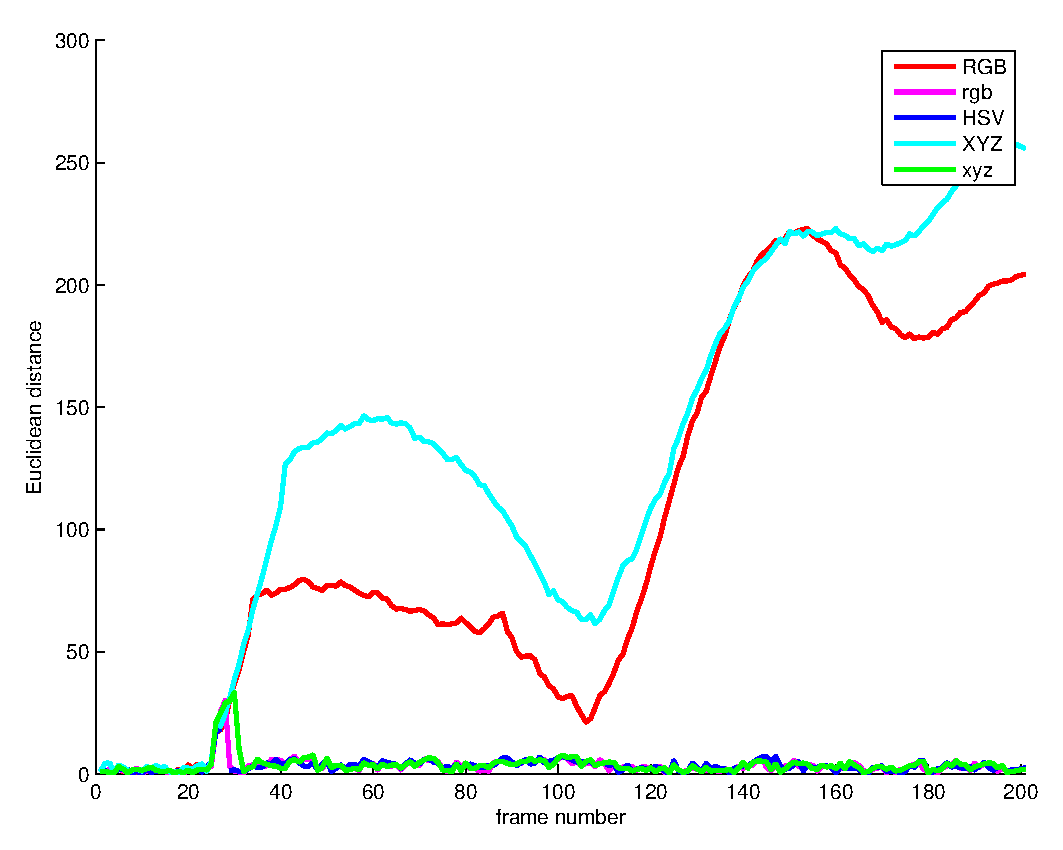
\includegraphics[height=6.0cm]{img/soccer_orange_15625}
\label{fig:d}
}
\caption{Each graph shows the performance of the six different colormodels for
a number of bins on the soccer movie when tracking the orange player. All four
graphs show a very distinctive pattern on the colormodels that lost track, this
is the result of occlusion caused by a white player. The white player walks in
front of the orange target and pushes the model away at which point it finds a
new orange player and starts tracking him.}
\label{fig:soccer}
\end{figure}

\newpage
\section{Conclusions}
This report introduced an implementation of the mean shift tracking algorithm
together with various colormodels applied to videos from two different domains.
From the results we conclude that a significant histogramsize should be chosen
to represent a model for robust tracking. An insufficient amount of bins
overgeneralizes the model, at which point the tracker loses its target as
target and background are (according to the model) indistinguishable.
Furthermore the best colormodel, according to our results, is the normalized
$rgb$ model. That is, the $rgb$ colormodel had the best overall performance across
the domains and various histogramsizes.


\section{Future Work}
A lot can be improved in the current implementation. Some of these improvements
are:
\begin{itemize}
\item{\emph{Scale}, compute the Epanechnikov kernel for various scales and
select the best scale for each frame using the Bhattacharyya distance.}
\item{\emph{Kalman}, improve the tracker by applying a Kalman filter to get
(even) better approximations in future frames.}
\item{\emph{Color}, on the manual selection of the object to track, one could
perform some analysis to determine which color space is best suited for the
target model. For example the color space model with the highest variance coul
be used.}
\item{\emph{Spatial}, divide the kernel into several parts to store spatial
information for more discriminative models.}
\end{itemize}
Unfortunatly, due to time constraints we were not able to apply these kind of
improvements.

\renewcommand\bibname{References}
\bibliography{references}
\bibliographystyle{IEEEtran}
\end{document}
